\documentclass[14pt,xcolor=pdftex,dvipsnames,table]{beamer}\usepackage[]{graphicx}\usepackage[]{color}
%% maxwidth is the original width if it is less than linewidth
%% otherwise use linewidth (to make sure the graphics do not exceed the margin)
\makeatletter
\def\maxwidth{ %
  \ifdim\Gin@nat@width>\linewidth
    \linewidth
  \else
    \Gin@nat@width
  \fi
}
\makeatother

\definecolor{fgcolor}{rgb}{0.345, 0.345, 0.345}
\newcommand{\hlnum}[1]{\textcolor[rgb]{0.686,0.059,0.569}{#1}}%
\newcommand{\hlstr}[1]{\textcolor[rgb]{0.192,0.494,0.8}{#1}}%
\newcommand{\hlcom}[1]{\textcolor[rgb]{0.678,0.584,0.686}{\textit{#1}}}%
\newcommand{\hlopt}[1]{\textcolor[rgb]{0,0,0}{#1}}%
\newcommand{\hlstd}[1]{\textcolor[rgb]{0.345,0.345,0.345}{#1}}%
\newcommand{\hlkwa}[1]{\textcolor[rgb]{0.161,0.373,0.58}{\textbf{#1}}}%
\newcommand{\hlkwb}[1]{\textcolor[rgb]{0.69,0.353,0.396}{#1}}%
\newcommand{\hlkwc}[1]{\textcolor[rgb]{0.333,0.667,0.333}{#1}}%
\newcommand{\hlkwd}[1]{\textcolor[rgb]{0.737,0.353,0.396}{\textbf{#1}}}%

\usepackage{framed}
\makeatletter
\newenvironment{kframe}{%
 \def\at@end@of@kframe{}%
 \ifinner\ifhmode%
  \def\at@end@of@kframe{\end{minipage}}%
  \begin{minipage}{\columnwidth}%
 \fi\fi%
 \def\FrameCommand##1{\hskip\@totalleftmargin \hskip-\fboxsep
 \colorbox{shadecolor}{##1}\hskip-\fboxsep
     % There is no \\@totalrightmargin, so:
     \hskip-\linewidth \hskip-\@totalleftmargin \hskip\columnwidth}%
 \MakeFramed {\advance\hsize-\width
   \@totalleftmargin\z@ \linewidth\hsize
   \@setminipage}}%
 {\par\unskip\endMakeFramed%
 \at@end@of@kframe}
\makeatother

\definecolor{shadecolor}{rgb}{.97, .97, .97}
\definecolor{messagecolor}{rgb}{0, 0, 0}
\definecolor{warningcolor}{rgb}{1, 0, 1}
\definecolor{errorcolor}{rgb}{1, 0, 0}
\newenvironment{knitrout}{}{} % an empty environment to be redefined in TeX

\usepackage{alltt}

% Specify theme
\usetheme{Madrid}
% See deic.uab.es/~iblanes/beamer_gallery/index_by_theme.html for other themes
\usepackage{caption}
\usepackage[comma, sort&compress]{natbib}
\usepackage{graphicx}
\usepackage{amsmath}
\bibliographystyle{agsm}
% Specify base color
\usecolortheme[named=OliveGreen]{structure}
% See http://goo.gl/p0Phn for other colors

% Specify other colors and options as required
\setbeamercolor{alerted text}{fg=Maroon}
\setbeamertemplate{items}[square]

% Title and author information
\title{Tests of Residuals and Coefficients}
\author{Rob Hayward}
\IfFileExists{upquote.sty}{\usepackage{upquote}}{}


\begin{document}

\begin{frame}
\titlepage
\end{frame}

\begin{frame}{Outline}
\tableofcontents
\end{frame}

\section{Residual Tests}
Why Test Residuals? Part 2 p. 159
Assumptions for OLS to be BLUE
\begin{itemize}[<+-| alert@+>]
\item Residuals should be iid
\begin{itemize}
\item No auto or serial correlation: residuals are \emph{independent}
\item No Hetroskedasticity: residuals are \emph{identically distributed}
\end{itemize}
\item We would also like the residuals to be \emph{normally distributed}: so that we can use the known quantiles from the normal distribution to test assertions about the model
\end{itemize}


\begin{frame}{View a normal random variable}
\graphicspath{{./Figures/}}
\frametitle{View a normal random variable}
\begin{center}
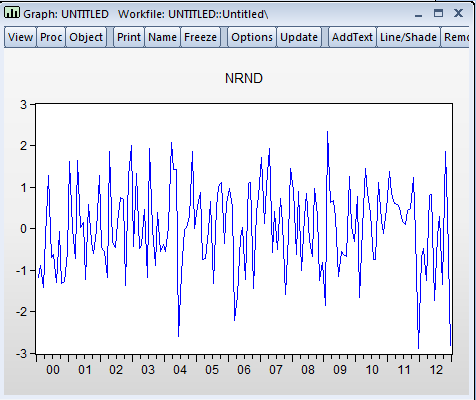
\includegraphics[height = 3.0in]{NRND}
\end{center}
\end{frame}

\begin{frame}{View Residuals}
\graphicspath{{./Figures/}}

\frametitle{View Residuals}
\begin{center}
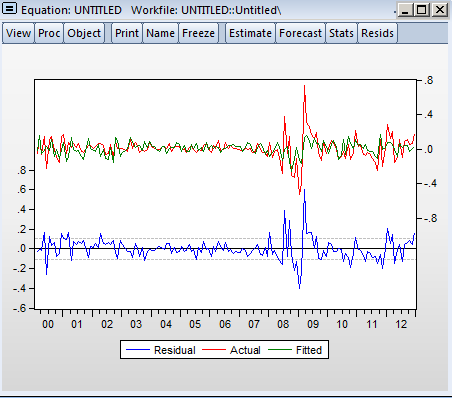
\includegraphics[height = 3.0in]{Resid}
\end{center}
\end{frame} 

\subsection{Autocorrelation}
\begin{frame}{Testing Autocorrelation}
The test for serial correlation is 
\begin{equation*}
\tau_k = \frac{\sum_{t = k + 1}^T (Y_t - \bar{Y})(Y_{t - k} - \bar{Y})}{\sum_{t= 1}^T (Y_t - \bar{Y})^2}
\end{equation*}
where $k$ is the number of lags, $T$ the number of observations and $\bar{Y}$ is the mean of the variable. 
\end{frame}

\begin{frame}{Correlogram Part 1 p. 334}
\graphicspath{{./Figures/}}
%\frametitle{View Residuals}
\begin{center}
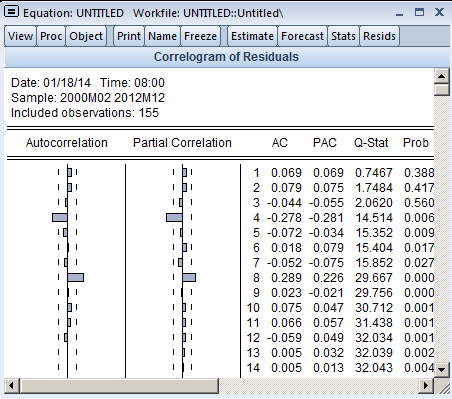
\includegraphics[height = 3.0in]{Corr}
\end{center}


\begin{frame}{Autocorrelation test}
Autocorrelation test
\begin{itemize}[<+-| alert@+>]
\item The null hypthesis $(H0)$ is of \emph{No autocorrelation}
\item The \emph{critical values} are estimated as $\pm 2/ \sqrt{T}$
\item $PAC_k$ is regression of $Y_t$ on $Y_k$ and other lags
\begin{itemize}
\item $Y_t = \beta_0 + \beta_1 Y_{t-1} + \beta_1 Y_{t-2} + \varepsilon$
\end{itemize}
\item Q-statistic.  Also tests no autocorrelation 
\begin{itemize}
\item $Q = T(T + 2) \sum_{J = 1}{k} \frac{\tau^2}{T - J}$
\item It is a $\chi^2$ test with p-values for critical values supplied
\end{itemize}
\end{itemize}
\end{frame}

\subsection{Hetroskedasticity}
\begin{frame}{Hetroskedasticity}
Is the variance constant? 
\begin{itemize}[<+-| alert@+>]
\item Financial time series often show volatilty clustering
\begin{itemize}
\item Try to model volatility (i.e. GARCH)
\end{itemize}
\item Variance may also change over the sample due to things like measurement
\begin{itemize}
\item For example, income increases over time, therefore attempts to model income are likely to encounter increased variance in the errors
\item Use logs to try to make changes in income proportional across sample
\end{itemize}
\end{itemize}
\end{frame}

\begin{frame}{Hetroskedasticity Tests}
There are a number of tests.  They tend to test whether the residuals are related to each other or time
\begin{itemize}[<+-| alert@+>]
\item LM Test
\begin{itemize}
\item $u_t^2 = \beta_0 + \beta_1 X_{1, t} + \beta_2 X_{2, t} + v_t$
\end{itemize}
\item Arch Test
\begin{itemize}
\item $u_t^2 = \beta_0 + \beta_1 u_{t-1}^2 + v$
\end{itemize}
\end{itemize}
\end{frame}


\begin{frame}{Brusch-Pagan-Godfrey}
\graphicspath{{./Figures/}}
%\frametitle{View Residuals}
\begin{center}
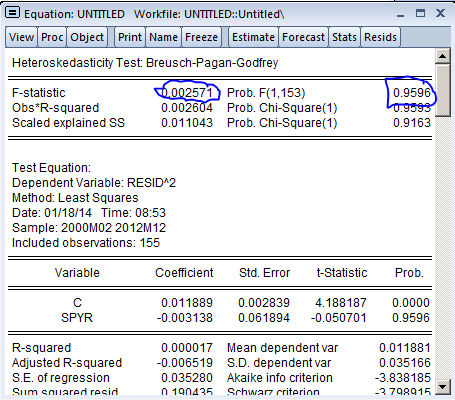
\includegraphics[height = 3.0in]{Hetf}
\end{center}
\end{frame} 


\section{Coefficient Tests}
\begin{frame}{Coefficient test}
Make tests of values of coefficients
\begin{itemize}[<+-| alert@+>]
\item We already tested whether coefficient values are zero using the t-test
\item One-sided test of sign on coefficient (postive or negative)
\item T-test can be extended to tests of other values
\begin{itemize}
\item $\text{t-stat} = \frac{\text{estimator} - \text{hypothesised value}}{\text{standard error of the estimator}}$\\ 
\item $t = \frac{\hat{\beta_1}-\beta_{1,}}{SE(\hat{\beta_1})}$\\
\end{itemize}
\end{itemize}
\end{frame}

\begin{frame}{Broader Restrictions}
Broader tests of the value of the coefficients can be made with the \emph{F-test}.  
\begin{block}{}
This will compare the RSS for the \emph{Restricted Model} with the RSS in the \emph{Unrestrcted Model}
\end{block}
\begin{itemize}[<+-| alert@+>]
\item $F = \frac{RSS_r-RSS_{ur}/T}{RSS_{ur}/(T - k)}$
\begin{itemize}
\item $RSS_r$ is the Residual Sum of Squares of the \emph{restricted model}
\item $RSS_{ur}$ is the Residual Sum of Squares of the \emph{unrestricted model}
\item T is the number of observations in the sample
\item k is the number of restrictions. 
\end{itemize}
\item This statistic has an F-distribution.  Called a \emph{Wald Test}
\end{itemize}
\end{frame}

\begin{frame}{F-test of zero coefficients}
\graphicspath{{./Figures/}}
%\frametitle{View Residuals}
\begin{center}
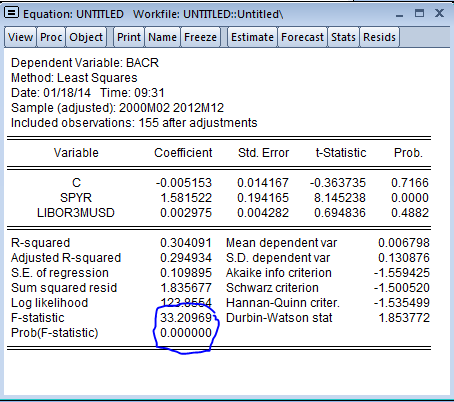
\includegraphics[height = 3.0in]{F-test}
\end{center}
\end{frame} 


\end{document}
